
\begin{document}

\abstract{Un sistema de inteligencia de negocio está formado por diferentes elementos, pero de todas las piezas la principal de ellas es el datawarehouse o almacén de datos, ya que es el componente que almacena los datos a analizar. En este capítulo vamos a explicar qué es un data warehouse, cómo se cargan los datos en el datawarehouse mediante los procesos de Extracción, Transformación y Carga (ETL) y cómo se pueden consultar los datos de la data warehouse de forma fácil, eficiente y potente mediante tecnologías OLAP.

Seguramente han escuchado muchas veces el término de Data Warehouse; podemos definirla como una base de datos corporativa donde se integra y depura información de una o varias fuentes distintas, que luego serán procesadas y analizadas desde distintos puntos de vista con afinidad de perspectivas y grandes velocidades de respuesta.

La creación del Data Warehouse representa la mayoría de las veces el primer paso, desde el punto de vista técnico, para implantar una solución completa y fiable de Business Intelligence y así aportar las mejores respuestas a los problemas de la organización.

Por otro lado, vemos al Datalake es un repositorio de almacenamiento que contienen una gran cantidad de datos en bruto y que se mantienen allí hasta que sea necesario. A diferencia de un data warehouse jerárquico que almacena datos en ficheros o carpetas, un datalake utiliza una arquitectura plana para almacenar los datos.
}

\abstract{
A business intelligence system is made up of different elements, but all the main parts of them are the data warehouse or the data warehouse, and the component that stores the data to be analyzed. In this chapter we will explain what a data warehouse is, how data is loaded in the data warehouse, extraction processes, Transformation and Loading (ETL) and how data warehouse data can be consulted easily, efficiently and powerful through OLAP technologies.

Surely you have heard the term Data Warehouse many times; We can define it as a corporate database where information is integrated and filtered from several different sources, which are then processed and analyzed as points of view with affinity of perspectives and great response speeds.

The creation of the Data Warehouse represents most of the time the first step, from the technical point of view, to implement a complete and reliable solution of Business Intelligence and thus also the best answers to the problems of the organization.

On the other hand, we see Datalake is a storage repository that contains a large amount of raw data and that stays there until the sea is necessary. A difference of a data store that stores data in folders or files, a data lake uses a flat architecture to store the data.}

\newpage

\section{Introduccion}
\item{Internet y las nuevas tecnologías han provocado el acceso y el almacenamiento desmesurado de información de los clientes y potenciales. Las empresas son cada vez más conscientes de la importancia que tienen esos datos para conocer mejor a los usuarios y así poder ofrecerles aquello que realmente piden, y no lo que nosotros pensamos que necesitan.\\\\
Esto es lo que se llama, aplicar estrategias customer centric. Para ello se necesita gestionar altos volúmenes de datos, tanto en tiempo real como organizados. Para ello, no hay nada mejor que un Data Warehouse o un Data Lake. Si no sabes exactamente en qué consisten, no te preocupes, en este post te cuento de una manera sencilla, qué son, para qué sirven y las principales ventajas, ¿vamos a por ello?\\\\
El término de Data Warehouse fue acuñado por Bill Inmon, traduciéndose literalmente como Almacén de Datos. Sin embargo, si fuera meramente un almacén de datos, no solucionaría el principal problema por el que se creó, estructurar de una manera lógica la información, con el objetivo de poder construir consultas que aporten información de valor al analista de datos.}

\newpage


\section{DATAWAREHOUSE}
\item{Algunas definiciones de Data Warehouse.

Un almacén de datos (Data Warehouse) es una colección de datos orientada a un determinado ámbito (empresa, organización, etc.), integrado, no volátil y variable en el tiempo, que ayuda a la toma de decisiones en la entidad en la que se utiliza. Es una estructura de datos donde la información contenida esta diseñada para favorecer el análisis y la divulgación eficiente de datos. Los almacenes de datos contienen a menudo grandes cantidades de información que se subdividen a veces en unidades lógicas más pequeñas dependiendo del subsistema de la entidad del que procedan o para el que sean necesario. Dichas unidades se denominan Data Marts.

Un Data Warehouse es una Base de Datos que contiene:

Datos empresariales

Integrar colección de datos históricos

Datos: dirigidos al usuario, consolidados y consistentes

Datos estructurados para distribución y consultas

Un Data Warehouse es un repositorio de datos de muy fácil acceso, alimentado de numerosas fuentes, transformadas en grupos de información sobre temas específicos de negocios, para permitir nuevas consultas, análisis, reportes y decisiones.

Existen dos grandes autores con respecto al tema Data Warehouse: Bill Inmon y Ralph Kimball.

Bill Inmon: "El Data Warehouse es una colección de datos orientados al tema, integrados, no volátiles e historiados, organizados para el apoyo de un proceso de ayuda a la decisión"

Ralph Kimball: "El Data Warehouse es una copia de las transacciones de datos específicamente estructurada para la consulta y el análisis; es la unión de todos los Data Marts de una entidad".
\textbf{Caracteristicas}\\\\
•	Los datos almacenados en el Data Warehouse deben integrarse en una estructura consistente. La información, además, debe estructurarse en diferentes niveles, adecuándose a las necesidades de cada uno de los usuarios.\\
•	Los datos se deben de organizar por temas para facilitar su acceso y entendimiento por parte de los usuarios. Por ejemplo, todos los datos sobre ventas, deben de estar almacenados en el mismo sitio, de tal modo que, al realizar la consulta sobre ventas, sea más sencillo.\\
•	Los datos suelen representar una situación en un momento presente, sin embargo, el Data Warehouse debe de cargarse con los distintos valores que toma una variable en el tiempo para permitir analizar las tendencias y crear un histórico.\\
•	La información que se almacena en un Data Warehouse es permanente y no debe ser modificada. Se deben de incorporar nuevos valores de las mismas variables, sin realizar ninguna acción sobre las ya existentes. De este modo podemos sacar conclusiones.\\\\
Sin embargo, el objetivo último del Data Warehouse, no es otro que facilitar el procesamiento de datos, con el fin de analizar dicha información desde diferentes puntos de vista y a gran velocidad.\\\\
Para ello, es fundamental poder realizar un análisis multidimensional. De este modo, si queremos conocer el número de ventas del modelo de zapatillas X, color azul, de la tienda de la calle Real, en La Coruña, del año 2016 al año 2018, disponiendo de un Data Warehouse, el proceso es sencillo, ya que previamente hemos realizado una jerarquización de la información y creado diferentes dimensiones.\\\\
Otra característica importante del Data Warehouse, son los metadatos, ¿qué es esto? Muy sencillo. Imagínate que tienes una serie de datos almacenados, pero no sabes de dónde proceden, cuándo se incluyeron, su fiabilidad, la forma de calcularlos… Con los metadatos tienes toda esa información. Estos metadatos son también los responsables de que se puedan construir consultas, informes o análisis.

}

\section{VENTAJAS}
\item{\textbf{Principales ventajas del uso de un Data Warehouse}\\\\
Estas son las principales ventajas que se pueden encontrar en la implantación de un Data Warehouse en el proceso de gestión del dato en tu negocio:\\\\
•	Facilita la toma de decisiones basadas en datos, en cualquier área funcional de la empresa, ya que te proporciona información integrada y global del negocio.\\
•	La información se convierte en un valor añadido para cualquier negocio, gracias a que permite aplicar técnicas estadísticas de análisis y modelización que ayudan a encontrar relaciones ocultas entre los datos almacenados.\\
•	Te permite de manera sencilla aprender de los datos del pasado y predecir situaciones futuras para diferentes escenarios.\\
•	Simplifica la implantación de sistemas de gestión integral de la relación con el cliente, dentro de la empresa.\\
•	Supone una optimización tecnológica y económica en entornos de Centro de Información, estadística o de generación de informes con retornos de la inversión espectaculares.\\
•	Es un sistema especialmente útil para el medio y el largo plazo.\\
•	Aumenta la productividad de las empresas de manera muy sustancial.
•	Te permite realizar planes de una manera mucho más efectiva.\\
•	Permite la integración de todas las herramientas corporativas. Por ejemplo, nosotros en Artyco integramos toda la información que recogemos a través de todas nuestras aplicaciones (monitorización web, crm, wifi tracking, campañas…) en un Data Warehouse, de donde sacar la información necesaria ante consultas determinadas.\\
•	Para trabajar de manera correcta un Data Warehouse, es preciso que todos los componentes de la organización hablen el mismo lenguaje, es decir, que todos llamen a las cosas por su nombre. De este modo, gracias al Data Warehouse se pueden unificar conceptos.

}

\section{DATALAKE}
\item{Un Data Lake no es otra cosa que un gran almacén de datos en bruto, los cuales se mantienen tal cual han llegado, y hasta que se necesitan para su uso. La principal diferencia con el Data Warehouse, está en la jerarquía y el almacenamiento de los datos en ficheros y carpetas que utiliza este, frente a la arquitectura plana del Data Lake. Podríamos decir que el Data Lake se nutre de Big Data y datos en tiempo real, tanto estructurados como no estructurados, en una amalgama plana, sobre la cual puedes recoger aquella información que necesites.\\\\
\textbf{Caracteristicas}\\\\
•	Permite una fácil y rápida búsqueda de datos. El Data Lake está asociado al Big Data, en el sentido de que es el recipiente donde descansan todos esos datos. Al no estar organizados como en el Data Warehouse, se hace necesaria una búsqueda eficiente de la información que en este se contiene. Esta búsqueda se realiza básicamente a través de machine learning.\\
•	Un Data Lake inteligente permite analizar eficazmente el grado de protección de la información que se guarda en los diferentes silos. Con la nueva normativa europea GDPR, esta seguridad en la privacidad de los datos se ve asegurada.\\
•	El Data Lake te permite ser rápido y disponer de datos en tiempo real. Además, te permite preparar y compartir rápidamente datos que son fundamentales para ofrecer analíticas competitivas.\\
•	Te permite guardar pasos de preparación de datos y luego reproducir rápidamente esos pasos dentro de procesos automatizados. Es decir, muchas veces los analistas repiten las mismas actividades en la preparación de datos. Con un Data Lake inteligente, puedes acceder a esos procesos y reducir tiempos y esfuerzos.
}
\section{BENEFICIOS}
\item{
\textbf{Principales beneficios de un Data Lake}\\\\
•	El Data Lake permite centralizar todos los datos en un mismo lugar, vengan de la fuente que vengan. Una vez incluidas en su silo correspondiente de información, pueden ser procesadas a través de herramientas de Big Data. Muchas veces, en esa disparidad de información, habrá datos que requieran un tratamiento especial en cuanto a seguridad. Gracias al Data Lake, este aspecto se puede solventar.\\
•	Puede que la fuente original del dato esté obsoleta o se haya desactivado, sin embargo, su contenido puede que siga siendo valioso para el análisis. A través del Data Lake, puedes acceder a dicha información.\\
•	Todo dato que llegue al Data Lake puede ser normalizado y enriquecido.\\
•	Los datos se preparan en función de la necesidad del momento. Esto permite reducir considerablemente los costes y los tiempos. En el Data Warehouse, por ejemplo, es necesaria dicha preparación.\\
•	Se puede acceder a la información y enriquecerla desde cualquier punto del planeta, por cualquier usuario autorizado por el Data Lake. Esto ayuda a la organización a recopilar más fácilmente los datos necesarios para la toma de decisiones.\\
•	Un Data Lake pone la información en manos de un mayor número de personas dentro de cualquier organización, aprovechándose mejor la empresa de ese conocimiento que adquieren dichos individuos.
}

\section{DIFERENCIAS ENTRE DATA WAREHOUSE Y DATA LAKE}
\item{
\textbf{Podemos resumirlas en cinco grandes diferencias}\\\\
•	Un Data Lake conserva todos los datos, no sólo los que podrían utilizarse actualmente, sino también aquello que podrían necesitarse en un futuro. En frente, está el Data Warehouse que estudia muy bien qué datos incluir, cuáles son las fuentes de los datos. Además, se necesita dedicar tiempo para entender el negocio y así perfilar los datos. El Data Warehouse al final, contiene un modelo de datos altamente estructurado, diseñado para la generación de informes. El Data Lake utiliza un hardware muy diferente al del Data Warehouse. En el Data Lake, la ampliación a terabytes y petabytes es mucho más económico que en el caso del Data Warehouse. Es por eso, que en este último se mira tanto qué datos son necesarios para cºonservar, y cuales eliminar, ya que supone un costoso almacenamiento.\\\\
•	Un Data Lake soporta todos los tipos de datos, es decir, en este se guardan todos los datos, independientemente de la fuente y la estructura, y además, se mantienen en su forma bruta, transformándolos sólo cuando van a ser utilizados. En el Data Warehouse los datos almacenados son muchos más críticos para el negocio y la realización de informes. Por ejemplo, los datos de imágenes, comentarios en redes sociales, textos, etc, no suelen ser tenidos en cuenta, ya que, como he comentado, su almacenamiento es muy costoso.\\\\
•	Los Data Lakes son más flexibles que los Data Warehouses. Uno de los mayores problemas que presenta un Data Warehouse, está en el momento que se necesita realizar un cambio importante. Todo cambio se convierte en una tarea realmente difícil, ya que adaptar un Data Warehouse supone invertir mucho tiempo en el desarrollo de la estructura del almacén. Hoy día, las organizaciones demandan respuestas rápidas a sus preguntas comerciales, y en muchos casos, no pueden esperar a que el Data Warehouse se adapte. En cambio, el Data Lake, al almacenar todos los datos en bruto, permite el acceso de cualquier usuario para que los explote y analice en función de sus necesidades, encontrando la manera de responder a sus preguntas a su ritmo.\\\\
•	El Data Warehouse te proporciona unos resultados más limpios, estructurados y fiables. Sin embargo, en el Data Lake, al disponer de datos en bruto y sin estructurar, al hacer las consultas, usuarios no demasiado cualificados, recibirán información rápida, pero no del todo precisa, tal y como la obtendrían de un Data Warehouse. Normalmente, para usuarios de perfil Data scientist, este problema no existe en el Data Lake, ya que ellos crean sus reglas y estructuran la información para preparar sus análisis y modelos. El verdadero problema reside en el 80 porciento del resto de usuarios, quienes simplemente buscan tener acceso a ciertos kpis diarios.\\\\
Tanto los Data Warehouses como los Data Lakes están destinados a convivir en las empresas que deseen basar sus decisiones en datos. Como habrás podido entender, ambos son complementarios, no sustitutivos, pudiendo ayudar a cualquier negocio a conocer mejor el mercado y el consumidor, de cara a poder realizar estrategias basadas en el conocimiento de estos, con comunicaciones cada vez más personalizadas, es decir, ser más customer centric.
}
\begin{center}

\includegraphics[width=14cm]{./Imagenes/imagen1}
\end{center}

\begin{center}
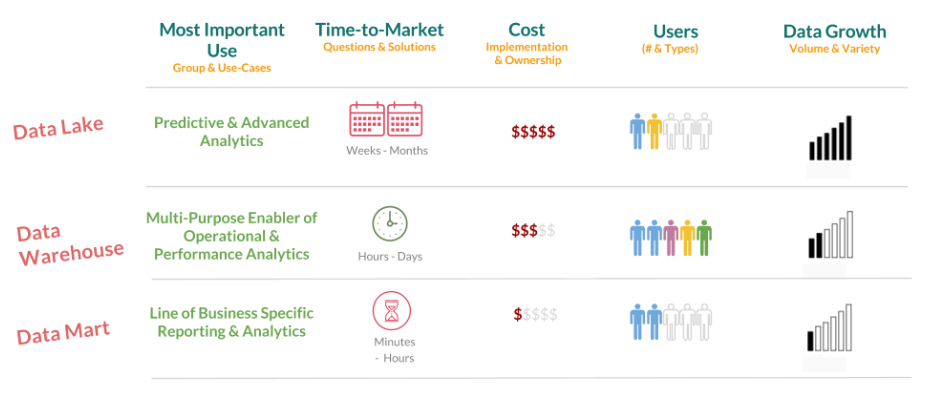
\includegraphics[width=14cm]{./Imagenes/imagen2}
\end{center}

\section{CONCLUSIONES}
\item{	El concepto de Data Warehouse abarca mucho más que simplemente copiar datos operacionales a una base de datos informacional distinta. El sistema deberá ofrecer una solución completa para gestionar y controlar el flujo de información desde bases de datos corporativas y fuentes externas a sistemas de soporte de decisiones de usuarios finales. Además, debe permitir a los usuarios conocer qué información existe en el almacén de datos, y cómo poder acceder a ella y manipularla.\\\\
	La discusión Data Lake vs Data Warehouse es algo muy común entre aquellas empresas que se disponen a implantar soluciones de big data. Rápidamente la conversación sobre datos y análisis en el ámbito de big data nos lleva al Data Lake o lago de datos, pero muy a menudo las empresas no acaban de entender bien qué es lo que esto significa y cuáles son las diferencias entre Data Lake vs Data Warehouse.\\\\
	De hecho, se pueden complementar muy bien, diseñando una arquitectura de datos moderna, que permita seguir a las organizaciones aprovechando sus inversiones en su Data Warehouse, mientras que empiezan a recoger en su Data Lake, todos los datos que han sido ignorados o desechados anteriormente.
}

\section{3.	RECOMENDACIONES }
\item{•	Debe enfocarse a toda la empresa: debe proveer información de todas las áreas de la empresa como ventas, finanzas, operación, etc.\\\\
•	El diseño debe ajustarse a los cambios: es decir que debe poder adaptarse al cambio de las reglas de negocio, permitiendo que el Data Warehouse debe seguir brindando información de soporte a decisiones en un nuevo contexto de las necesidades de la empresa.\\\\
•	Preparado para carga masiva de datos: El proceso de carga no debe ser extenso en complejidad y tiempo de ejecución, se deben aplicar todas las técnicas de gestión especializada de datos de manera de tener un proceso eficiente. Recordemos que estos sistemas están diseñados preferentemente para el análisis de la información, es de decir, la obtención de indicadores o KPI.\\\\
•	Debe ser multipropósito: Su diseño debe ser fácil de entender, de escalar y de actualizar, de manera de estar preparado para todas las formas posibles análisis de Business Intelligence.
}

% Bibliografía.
%-----------------------------------------------------------------
\begin{thebibliography}{99}
•	https://blog.powerdata.es/el-valor-de-la-gestion-de-datos/data-lake-vs-data-warehouse.-veamos-sus-principales-diferencias\\\\
•	https://tableauperu.com/data-warehouse/\\\\
•	https://blog.powerdata.es/el-valor-de-la-gestion-de-datos/data-lake-vs-data-warehouse.-veamos-sus-principales-diferencias\\\\
•	https://trends.inycom.es/principales-diferencias-data-lakes-data-warehouse/\\\\
•	pg 21 Thank	you! See	you	Thursday,	March	2 for	the	next webinar, Descriptive,	Prescriptive and	Predictive	Analytics John Ladley @jladley john@firstsanfranciscopartners.com\\\\
•	KO’Neal @kellezoneal kelle@firstsanfranciscopartners.com © 2016 First San Francisco Partners www.firstsanfranciscopartners.com

\bibitem{Cd94} Autor, \emph{Título}, Revista/Editor, (año)

\end{thebibliography}

\end{document}
